\section{Experiment Design}
\label{sec:experiment}

This section describes the experiment design. The study was approved by the university's Institutional Review Board (IRB). 

\subsection{Participant Recruitment}
This study recruited 202 Amazon Mechanical Turk (MTurk) participants after stratified sampling. Participants were first screened based on their age, gender, household income, and education level to assure a balanced demographic within each experiment condition while randomly assigning participants to these conditions. This approach aimed to mitigate imbalanced participation demographics~\cite{mturk_8}. We provide the demographic in Table X?

\begin{figure}[t]
    \centering
    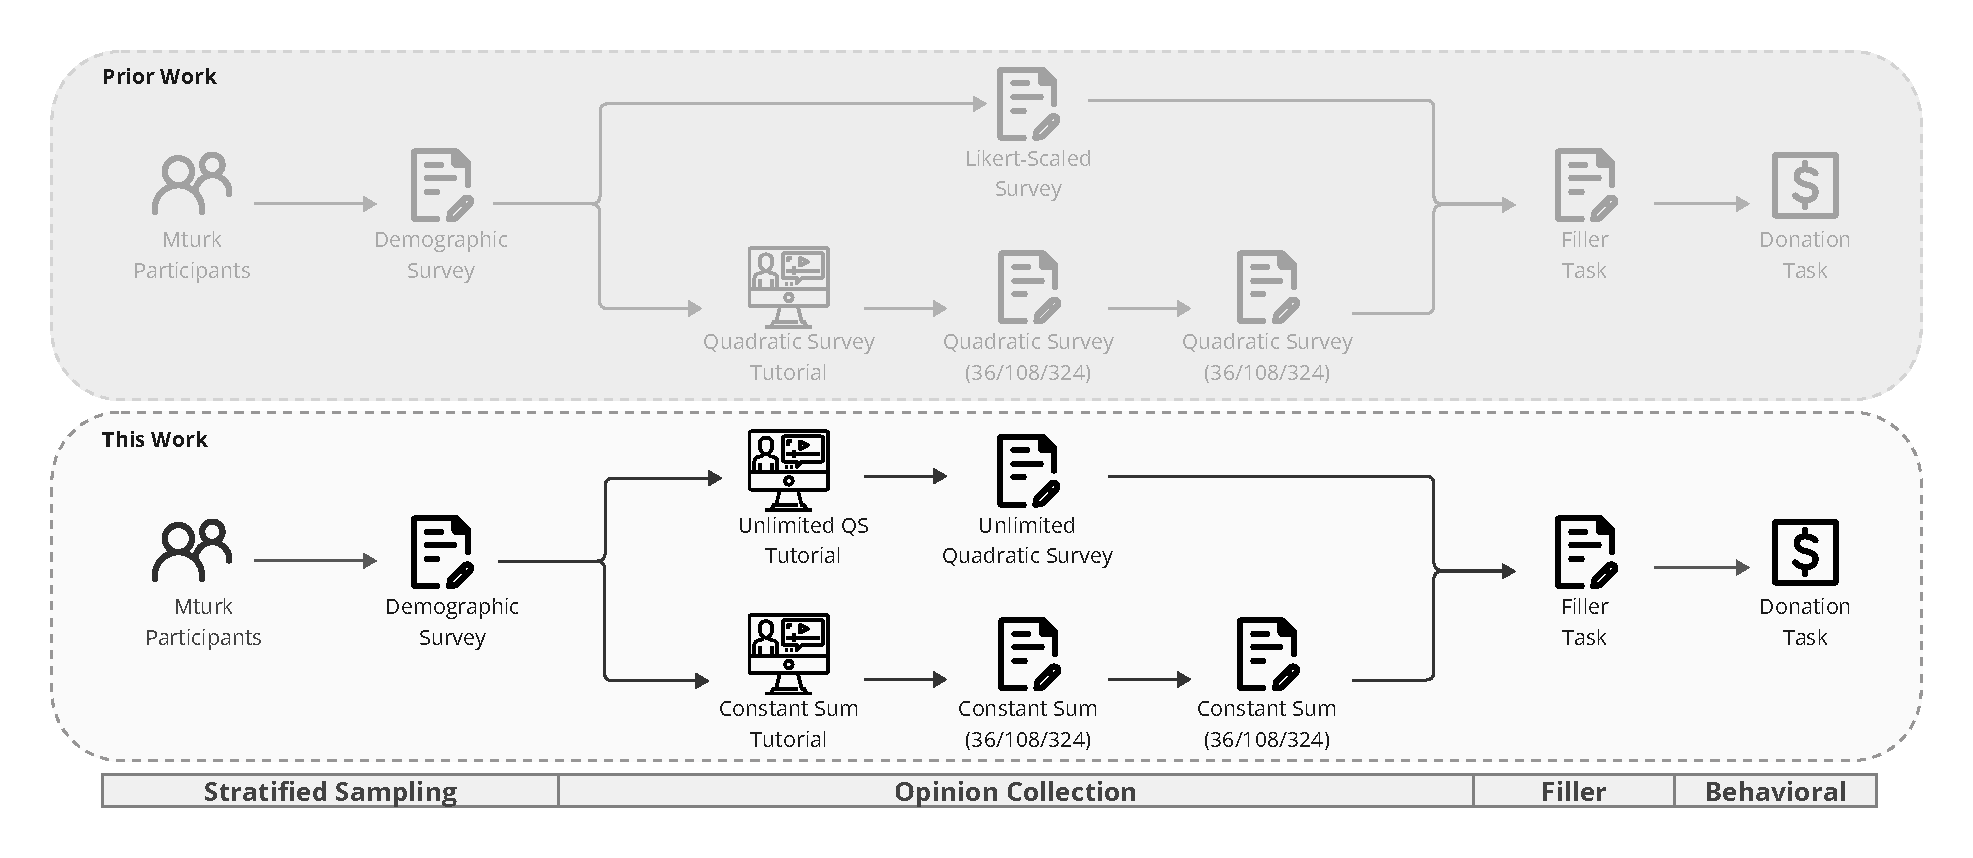
\includegraphics[width=\textwidth]{content/image/whyqs_exp_flow.pdf}
    \caption{Experiment overview. Our study covers the dotted box beneath, mirroring prior research only differing the type of surveys involved during the opinion collection section. The bar below highlights the four parts of the study: sampling, opinion collection, filler task, and the behavioral task.}
    \label{fig:experiment}
\end{figure}

\subsection{Experiment Design}
To ensure comparability with prior findings~\cite{chengCanShowWhat2021}, this study followed the same between-subject experimental design and altered the open sourced software to create two more conditions, creating four new experimental data. We highlight this addition in Figure~\ref{fig:experiment}. The four experiment conditions examine the effects of budget constraints and quadratic costs to answer RQ2. 

Four additional experimental conditions were introduced:  
\begin{itemize}
    \item **Unlimited QS (UQS):** Participants experience quadratic costs without budget constraints, isolating the effect of cost scaling.
    \item **Constant Sum Survey with 36 Credits (CS36):** A small-budget linear-cost condition testing the effect of budget constraints.
    \item **Constant Sum Survey with 108 Credits (CS108):** A medium-budget version allowing greater expressiveness.
    \item **Constant Sum Survey with 324 Credits (CS324):** A high-budget condition assessing whether increased budgets improve alignment.
\end{itemize}

The UQS condition isolates the effect of quadratic costs, while the CSS conditions isolate the effect of budget constraints. Together, these conditions allow for a direct comparison of cost mechanisms in preference elicitation. As mentioned in~\Cref{sec:related_works_css}, QS with linear cost function is slightly different then CSS where participants do not need to allocate all their provided credits, however, that effectly equals to an additional ``no response'' option on CSS, thus, here we denote these variations as CSS.

The system randomly assigned participants to the UQV group or the CSS group, where the it will assign the latter group two credit variations of CSS randomly. <report completion time> 

\subsubsection{Survey content}
Participants complete the 


% The experiment randomly assigned some of the
% participants to the Likert group, shown in the upper path of Figure 1. In the prompt, we explicitly
% told the participants that there are limited resources in society, and that people have different
% preferences at allocating resources to various societal causes. The survey focused on nine societal
% issues, including 1) pets and animals, 2) arts, culture and humanities, 3) education, 4) environment,
% 5) health, 6) human services, 7) international causes, 8) faith and spiritual causes, and 9) veterans4.
% We derived the nine societal causes from the categorization of charity groups on Amazon Smile5, a
% popular donation website that has accumulated over 100 million dollars of donations.
% We asked the participants to rate each of the nine societal issues on a 5-point Likert scale: “For
% each of the issues listed below, how important do you think the issue is to you and that more effort
% and resources should be contributed towards the issue?”. The 5-point Likert options ranged from
% “Very important” to “Very Unimportant.” While there are a variety of Likert scales (3-point, 5-point,
% 7-point, and even 11-point), we used a 5-point Likert scale since it is one of the most commonly
% used scale [16].

% The QV group took the lower path in Figure 1. We first asked
% participants to watch a pre-recorded tutorial video that introduced how QV works and how to
% use our QV interface since we did not expect participants to know about QV before taking part
% in the study, as opposed to Likert scale. Participants had unlimited time to interact with a demo
% QV interface to familiarize themselves with QV. To ensure that the participants paid attention

% and understood QV, they needed to correctly answer at least three of the five multiple-choice quiz
% questions related to QV to continue with the study.
% Once they passed the quiz, participants encountered two of the three versions of the QV surveys
% at random. The three versions of QV had 36, 108, and 324 voice credits, respectively. We showed
% them the same prompt as in the Likert group and instructed them to answer the same question
% for the nine identical causes, but with QV instead. Participants cast positive votes for causes they
% considered important and vice versa.
% To our knowledge, no prior work discussed about how to decide on the voice credit budget in QV
% empirically. Therefore, we designed three versions of the QV survey to answer the second question
% in RQ1: how does the amount of voice credits in QV impact QV’s ability to elicit true preferences?
% To examine how larger voice credit budgets impact people’s choices, we set an exponential increase
% based on the number of options (��) on the survey (�� (��), �� (��1.5) to �� (��2)). We investigated three
% levels of voice credits: �� × ��, ��1.5 × ��, and ��2 × ��, where �� is the number of options in the survey
% and �� is the number of credits required to express an attitude in QV that is equivalent to the
% strongest attitude in a 5-point Likert scale survey, where “Neutral" in Likert = 0 vote in QV and one
% level in Likert = one vote in QV. In this experiment, �� = 9 corresponded to the 9 societal causes.
% We used a 5-point Likert scale survey with extreme levels at ±2; hence each participant needed
% four voice credits (22 = 4) to express the extreme Likert levels in QV, which translated to �� = 4.
% Thus, the three levels of voice credits in the experiment were 9 × 4 = 36 (QV36), 91.5 × 4 = 108
% (QV108), and 92 × 4 = 324 (QV324). In all three cases, participants could afford to express any results
% from Likert in the form of QV. In addition, we asked participants to complete two of the three QV
% surveys to help understand how an increase or decrease in voice credits impacted their response
% behavior. To minimize the learning effects between the two versions, we provided participants a
% playground to get familiar with the QV interface and mechanism before taking the surveys. We
% randomized the order of the two versions.


\subsection{Experiment Design}
We implemented a between-subject design to avoid learning effects and minimize participants' fatigue from potential complexity of QSs. The experiment focused on public resource allotment, following the methodology of~\citet{chengCanShowWhat2021}, in which participants expressed preferences across societal issues. These issues are relevant to all citizens and effectively highlight the need to prioritize limited public resources. Participants received a survey with options randomly drawn from the 31 societal topics evaluated by Charity Navigator~\cite{charitynavigatorCharityNavigator2023}, an organization that assesses over 20,000 charities in the United States (see Appendix~\ref{sec:charityList} for the full list).
Randomly selecting the options each participant saw helped control for potential systematic content biases that specific voting options might introduce across surveys of different lengths. Participants were randomly assigned to one of four groups, each with 10 participants:
\begin{itemize}[leftmargin=*]
    \item Short Text (ST): A text interface with 6 options.
    \item Short Two-Phase (S2P): A two-phase interface 6 options.
    \item Long Text (LT): A text-based interface 24 options.
    \item Long Two-Phase (L2P): A two-phase interface with 24 options.
\end{itemize}

Prior research informed the choice of 6 and 24 options, representing short and long lists. These studies recommend fewer than 10 options for constant-sum surveys~\cite{moroneyQuestionnaireDesignHow2019} and fewer than 7 for the Analytic Hierarchy Process~\cite{saatyPrinciplesAnalyticHierarchy1987}. Classic cognitive load research~\cite{millerMagicalNumberSeven1956, saaty2003magic} suggests the use of 7$\pm$2 items. A meta-analysis by~\citet{chernevChoiceOverloadConceptual2015} identified 6 and 24 as common values for short and long lists in choice overload studies, which are rooted in the original choice overload experiment by~\citet{iyengarWhenChoiceDemotivating2000}.

\subsection{Experiment Procedure}
Participant's spent on average 40 minutes (range:~27$-$68,~$\sigma$=9) in the lab. Figure~\ref{fig:studyProtocol} visually represents the study protocol detailed in the following subsections.

\subsubsection{Consent, Instructions, and Quiz}
Participants were invited to the lab to control for external influences and used a 32-inch vertical monitor to display all options. After consenting, participants watched a video explaining the quadratic mechanism without any mention of the interface's operation, followed by a quiz to ensure understanding. Participants rewatched the video or consulted the researcher until they successfully selected the correct answers. Each participant's screen was captured throughout the study.

\subsubsection{Quadratic Survey}
The researcher informed participants that the study aimed to help local community organizers understand preferences on societal issues to improve resource allocation. Aware that their screens were being recorded, participants completed the survey independently inside a semi-enclosed space in the lab, without the researcher's presence. Once they completed the survey, participants notified the researcher.

\subsubsection{NASA-TLX Survey and Interview}
The researcher joins study participant and administer a paper-based weighted NASA Task Load Index (NASA-TLX), followed by a semi-structured interview after being informed that the researcher would begin audio recording with their laptop. We adopted the paper-based weighted NASA-TLX, a widely used multidimensional tool that averages six subscale scores to measure overall workload after task completion~\cite{hart1988development, hartNasaTaskLoadIndex2006, cain2007review}. NASA-TLX is favored for its low cost and ease of administration~\cite{gaoMentalWorkloadMeasurement2013}, and it exhibits less variability compared to one-dimensional workload scores~\cite{rubioEvaluationSubjectiveMental2004}, making it suitable for our study. 

While cognitive load can be assessed through psychophysiological, performance, subjective, and analytical measures~\cite{gaoMentalWorkloadMeasurement2013}, the length and complexity of QSs make some of these impractical. Performance and analytical measures require task switching or interruptions, which risk increasing overall cognitive load and experiment time. Psychophysiological measures, such as pupil size~\cite{palinkoEstimatingCognitiveLoad2010} and ECG~\cite{haapalainenPsychophysiologicalMeasuresAssessing2010}, are costly, sensitive to external factors, and often require participants to wear additional equipment.

\subsubsection{Demographic, Debrief, and Compensation}
After the interview, the researcher collected participant's demographics and debriefed them, explaining that the study's goal was to understand interface design and cognitive load. Participants received a \$15 cash compensation.

\subsection{Quantitative Measures: Clickstream Data}
\label{subsec:measures}

Besides using NASA-TLX and interviews to capture cognitive load, we also recorded participants' clickstream data from the interface (i.e., each click and the corresponding UI component). These log data enabled us to analyze how participants navigated and engaged with the survey options.

\paragraph{Edit Distance} We introduce three related metrics---edit distance per option, edit distance per action, and cumulative edit distance---to quantify the distance participants traveled across the interface. Edit distance per option sums the total number of options traversed while modifying a single vote option, edit distance per action measures the distance traversed during each individual adjustment, and cumulative edit distance captures the total distance traversed throughout the entire survey. The formal definitions and modeling approach are provided in~\Cref{sec:dist}.

\paragraph{Time Spent per Option} In addition, we computed the total time participants spent interacting with each specific option by aggregating the time spent on that specific option during the survey. We describe and discuss these findings in~\Cref{sec:timeAnalysis}.